% flashcards-title: Piecewise position-time graph
% flashcards-desc: Position rises from negative two metres at zero seconds to two metres at two seconds, stays at two metres until four seconds, then falls to negative one metre at six seconds.
\documentclass[border=7pt]{standalone}
\def\pgfsysdriver{pgfsys-dvisvgm.def}
\usepackage{tikz}
\usetikzlibrary{arrows.meta,positioning,shapes.geometric}
\definecolor{mechInk}{HTML}{172033}
\definecolor{mechBlue}{HTML}{155EEF}
\definecolor{mechOrange}{HTML}{B54708}
\definecolor{mechPale}{HTML}{E8F0FF}
\definecolor{mechGray}{HTML}{667085}
\definecolor{mechLight}{HTML}{D0D5DD}
\tikzset{
  every picture/.style={font=\sffamily\large, text=mechInk},
  mech box/.style={draw=mechInk, line width=1.2pt, rounded corners=4pt,
    fill=white, align=center, minimum height=14mm, inner xsep=5mm},
  mech primary/.style={draw=mechBlue, line width=2.2pt},
  mech secondary/.style={draw=mechOrange, line width=2.2pt, dashed},
  mech guide/.style={draw=mechGray, line width=0.9pt, dashed},
  mech arrow/.style={-{Stealth[length=3.2mm,width=2.4mm]},
    draw=mechInk, line width=1.4pt, line cap=butt},
  mech axis/.style={draw=mechInk, line width=1.2pt},
  mech tick/.style={draw=mechInk, line width=1pt}
}

\begin{document}
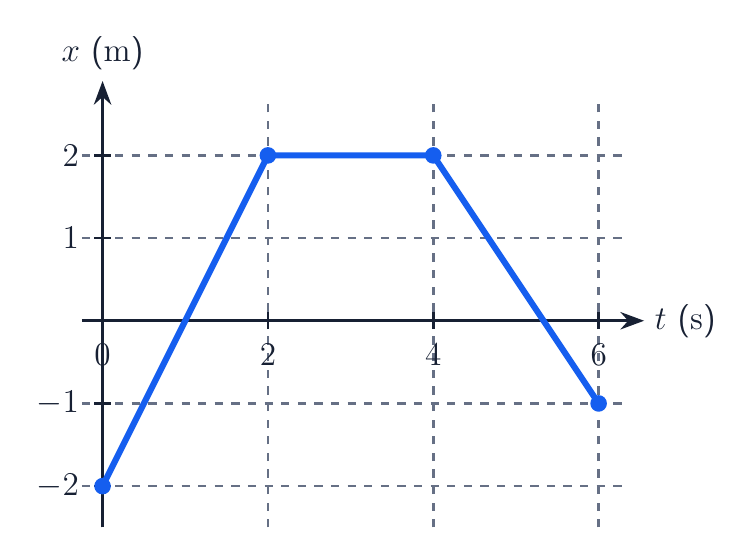
\begin{tikzpicture}[x=1.05cm,y=1.05cm]
  \foreach \x in {0,2,4,6} \draw[mech guide] (\x,-2.5) -- (\x,2.7);
  \foreach \y in {-2,-1,0,1,2} \draw[mech guide] (-0.25,\y) -- (6.35,\y);
  \draw[mech axis,-{Stealth[length=3mm,width=2.2mm]}] (0,-2.5) -- (0,2.9) node[above] {\(x\) (\(\mathrm{m}\))};
  \draw[mech axis,-{Stealth[length=3mm,width=2.2mm]}] (-0.25,0) -- (6.55,0) node[right] {\(t\) (\(\mathrm{s}\))};
  \foreach \x in {0,2,4,6} {
    \draw[mech tick] (\x,-0.1) -- (\x,0.1);
    \node[below=2pt] at (\x,-0.1) {\(\x\)};
  }
  \foreach \y in {-2,-1,1,2} {
    \draw[mech tick] (-0.1,\y) -- (0.1,\y);
    \node[left=2pt] at (-0.1,\y) {\(\y\)};
  }
  \draw[mech primary] (0,-2) -- (2,2) -- (4,2) -- (6,-1);
  \foreach \p in {(0,-2),(2,2),(4,2),(6,-1)} \fill[mechBlue] \p circle (3pt);
\end{tikzpicture}
\end{document}
